% Options for packages loaded elsewhere
\PassOptionsToPackage{unicode}{hyperref}
\PassOptionsToPackage{hyphens}{url}
\PassOptionsToPackage{dvipsnames,svgnames,x11names}{xcolor}
%
\documentclass[
]{article}

\usepackage{amsmath,amssymb}
\usepackage{iftex}
\ifPDFTeX
  \usepackage[T1]{fontenc}
  \usepackage[utf8]{inputenc}
  \usepackage{textcomp} % provide euro and other symbols
\else % if luatex or xetex
  \usepackage{unicode-math}
  \defaultfontfeatures{Scale=MatchLowercase}
  \defaultfontfeatures[\rmfamily]{Ligatures=TeX,Scale=1}
\fi
\usepackage{lmodern}
\ifPDFTeX\else  
    % xetex/luatex font selection
\fi
% Use upquote if available, for straight quotes in verbatim environments
\IfFileExists{upquote.sty}{\usepackage{upquote}}{}
\IfFileExists{microtype.sty}{% use microtype if available
  \usepackage[]{microtype}
  \UseMicrotypeSet[protrusion]{basicmath} % disable protrusion for tt fonts
}{}
\makeatletter
\@ifundefined{KOMAClassName}{% if non-KOMA class
  \IfFileExists{parskip.sty}{%
    \usepackage{parskip}
  }{% else
    \setlength{\parindent}{0pt}
    \setlength{\parskip}{6pt plus 2pt minus 1pt}}
}{% if KOMA class
  \KOMAoptions{parskip=half}}
\makeatother
\usepackage{xcolor}
\usepackage[margin=1in]{geometry}
\setlength{\emergencystretch}{3em} % prevent overfull lines
\setcounter{secnumdepth}{5}
% Make \paragraph and \subparagraph free-standing
\makeatletter
\ifx\paragraph\undefined\else
  \let\oldparagraph\paragraph
  \renewcommand{\paragraph}{
    \@ifstar
      \xxxParagraphStar
      \xxxParagraphNoStar
  }
  \newcommand{\xxxParagraphStar}[1]{\oldparagraph*{#1}\mbox{}}
  \newcommand{\xxxParagraphNoStar}[1]{\oldparagraph{#1}\mbox{}}
\fi
\ifx\subparagraph\undefined\else
  \let\oldsubparagraph\subparagraph
  \renewcommand{\subparagraph}{
    \@ifstar
      \xxxSubParagraphStar
      \xxxSubParagraphNoStar
  }
  \newcommand{\xxxSubParagraphStar}[1]{\oldsubparagraph*{#1}\mbox{}}
  \newcommand{\xxxSubParagraphNoStar}[1]{\oldsubparagraph{#1}\mbox{}}
\fi
\makeatother


\providecommand{\tightlist}{%
  \setlength{\itemsep}{0pt}\setlength{\parskip}{0pt}}\usepackage{longtable,booktabs,array}
\usepackage{calc} % for calculating minipage widths
% Correct order of tables after \paragraph or \subparagraph
\usepackage{etoolbox}
\makeatletter
\patchcmd\longtable{\par}{\if@noskipsec\mbox{}\fi\par}{}{}
\makeatother
% Allow footnotes in longtable head/foot
\IfFileExists{footnotehyper.sty}{\usepackage{footnotehyper}}{\usepackage{footnote}}
\makesavenoteenv{longtable}
\usepackage{graphicx}
\makeatletter
\def\maxwidth{\ifdim\Gin@nat@width>\linewidth\linewidth\else\Gin@nat@width\fi}
\def\maxheight{\ifdim\Gin@nat@height>\textheight\textheight\else\Gin@nat@height\fi}
\makeatother
% Scale images if necessary, so that they will not overflow the page
% margins by default, and it is still possible to overwrite the defaults
% using explicit options in \includegraphics[width, height, ...]{}
\setkeys{Gin}{width=\maxwidth,height=\maxheight,keepaspectratio}
% Set default figure placement to htbp
\makeatletter
\def\fps@figure{htbp}
\makeatother

\usepackage{graphicx}
\DeclareGraphicsExtensions{.png,.pdf,.jpg}
\usepackage{float}
\usepackage[section]{placeins}
\makeatletter
\@ifpackageloaded{tcolorbox}{}{\usepackage[skins,breakable]{tcolorbox}}
\@ifpackageloaded{fontawesome5}{}{\usepackage{fontawesome5}}
\definecolor{quarto-callout-color}{HTML}{909090}
\definecolor{quarto-callout-note-color}{HTML}{0758E5}
\definecolor{quarto-callout-important-color}{HTML}{CC1914}
\definecolor{quarto-callout-warning-color}{HTML}{EB9113}
\definecolor{quarto-callout-tip-color}{HTML}{00A047}
\definecolor{quarto-callout-caution-color}{HTML}{FC5300}
\definecolor{quarto-callout-color-frame}{HTML}{acacac}
\definecolor{quarto-callout-note-color-frame}{HTML}{4582ec}
\definecolor{quarto-callout-important-color-frame}{HTML}{d9534f}
\definecolor{quarto-callout-warning-color-frame}{HTML}{f0ad4e}
\definecolor{quarto-callout-tip-color-frame}{HTML}{02b875}
\definecolor{quarto-callout-caution-color-frame}{HTML}{fd7e14}
\makeatother
\makeatletter
\@ifpackageloaded{caption}{}{\usepackage{caption}}
\AtBeginDocument{%
\ifdefined\contentsname
  \renewcommand*\contentsname{Table of contents}
\else
  \newcommand\contentsname{Table of contents}
\fi
\ifdefined\listfigurename
  \renewcommand*\listfigurename{List of Figures}
\else
  \newcommand\listfigurename{List of Figures}
\fi
\ifdefined\listtablename
  \renewcommand*\listtablename{List of Tables}
\else
  \newcommand\listtablename{List of Tables}
\fi
\ifdefined\figurename
  \renewcommand*\figurename{Figure}
\else
  \newcommand\figurename{Figure}
\fi
\ifdefined\tablename
  \renewcommand*\tablename{Table}
\else
  \newcommand\tablename{Table}
\fi
}
\@ifpackageloaded{float}{}{\usepackage{float}}
\floatstyle{ruled}
\@ifundefined{c@chapter}{\newfloat{codelisting}{h}{lop}}{\newfloat{codelisting}{h}{lop}[chapter]}
\floatname{codelisting}{Listing}
\newcommand*\listoflistings{\listof{codelisting}{List of Listings}}
\makeatother
\makeatletter
\makeatother
\makeatletter
\@ifpackageloaded{caption}{}{\usepackage{caption}}
\@ifpackageloaded{subcaption}{}{\usepackage{subcaption}}
\makeatother

\ifLuaTeX
  \usepackage{selnolig}  % disable illegal ligatures
\fi
\usepackage{bookmark}

\IfFileExists{xurl.sty}{\usepackage{xurl}}{} % add URL line breaks if available
\urlstyle{same} % disable monospaced font for URLs
\hypersetup{
  pdftitle={Twitter and the Politics of the Federal Deficit},
  pdfauthor={Cy Coldiron},
  colorlinks=true,
  linkcolor={blue},
  filecolor={Maroon},
  citecolor={Blue},
  urlcolor={Blue},
  pdfcreator={LaTeX via pandoc}}


\title{Twitter and the Politics of the Federal Deficit}
\usepackage{etoolbox}
\makeatletter
\providecommand{\subtitle}[1]{% add subtitle to \maketitle
  \apptocmd{\@title}{\par {\large #1 \par}}{}{}
}
\makeatother
\subtitle{Results Summary}
\author{Cy Coldiron}
\date{2025-10-06}

\begin{document}
\maketitle

\renewcommand*\contentsname{Table of contents}
{
\hypersetup{linkcolor=}
\setcounter{tocdepth}{3}
\tableofcontents
}

\begin{tcolorbox}[enhanced jigsaw, colbacktitle=quarto-callout-important-color!10!white, arc=.35mm, bottomtitle=1mm, opacitybacktitle=0.6, title=\textcolor{quarto-callout-important-color}{\faExclamation}\hspace{0.5em}{Important}, rightrule=.15mm, breakable, left=2mm, coltitle=black, leftrule=.75mm, titlerule=0mm, colback=white, colframe=quarto-callout-important-color-frame, toprule=.15mm, toptitle=1mm, opacityback=0, bottomrule=.15mm]

\textbf{Writing sample disclaimer.} This PDF contains a draft of the
\emph{Results} section from the working paper\\
\textbf{Twitter and the Politics of the Federal Deficit}. The abstract
is included below for context.

\end{tcolorbox}

\subsection{Abstract (for context)}\label{abstract-for-context}

For decades, U.S political parties circumstantially exploit fears around
the the federal deficit to advance partisan goals. The shift to
social-media based political communication allows us to empirically
assess this long-held belief. Analyzing \textasciitilde3.6 million
tweets from official congressional accounts (June 2017--January 2023), I
identify deficit-related posts using a two-tier keyword approach and
estimate member--month logistic models linked to leadership roles and
legislative windows. Deficit rhetoric is uncommon overall---
\textbf{0.7\%} of tweets (≈7 per 1,000)---but varies sharply with
political context: Republicans tweet about the deficit five times as
often when in the minority, while Democrats' rates remain comparatively
stable across majority/minority status. Legislative periods further
amplify these patterns . The results confirm synchronized,
context-responsive messaging---especially for the GOP---and show that
deficit rhetoric is less a benchmark of fiscal conditions and operates
as a communication-weapon serving partisan ends.

\clearpage

\section{Macro Trends}\label{sec-macro}

\begin{figure}

\centering{

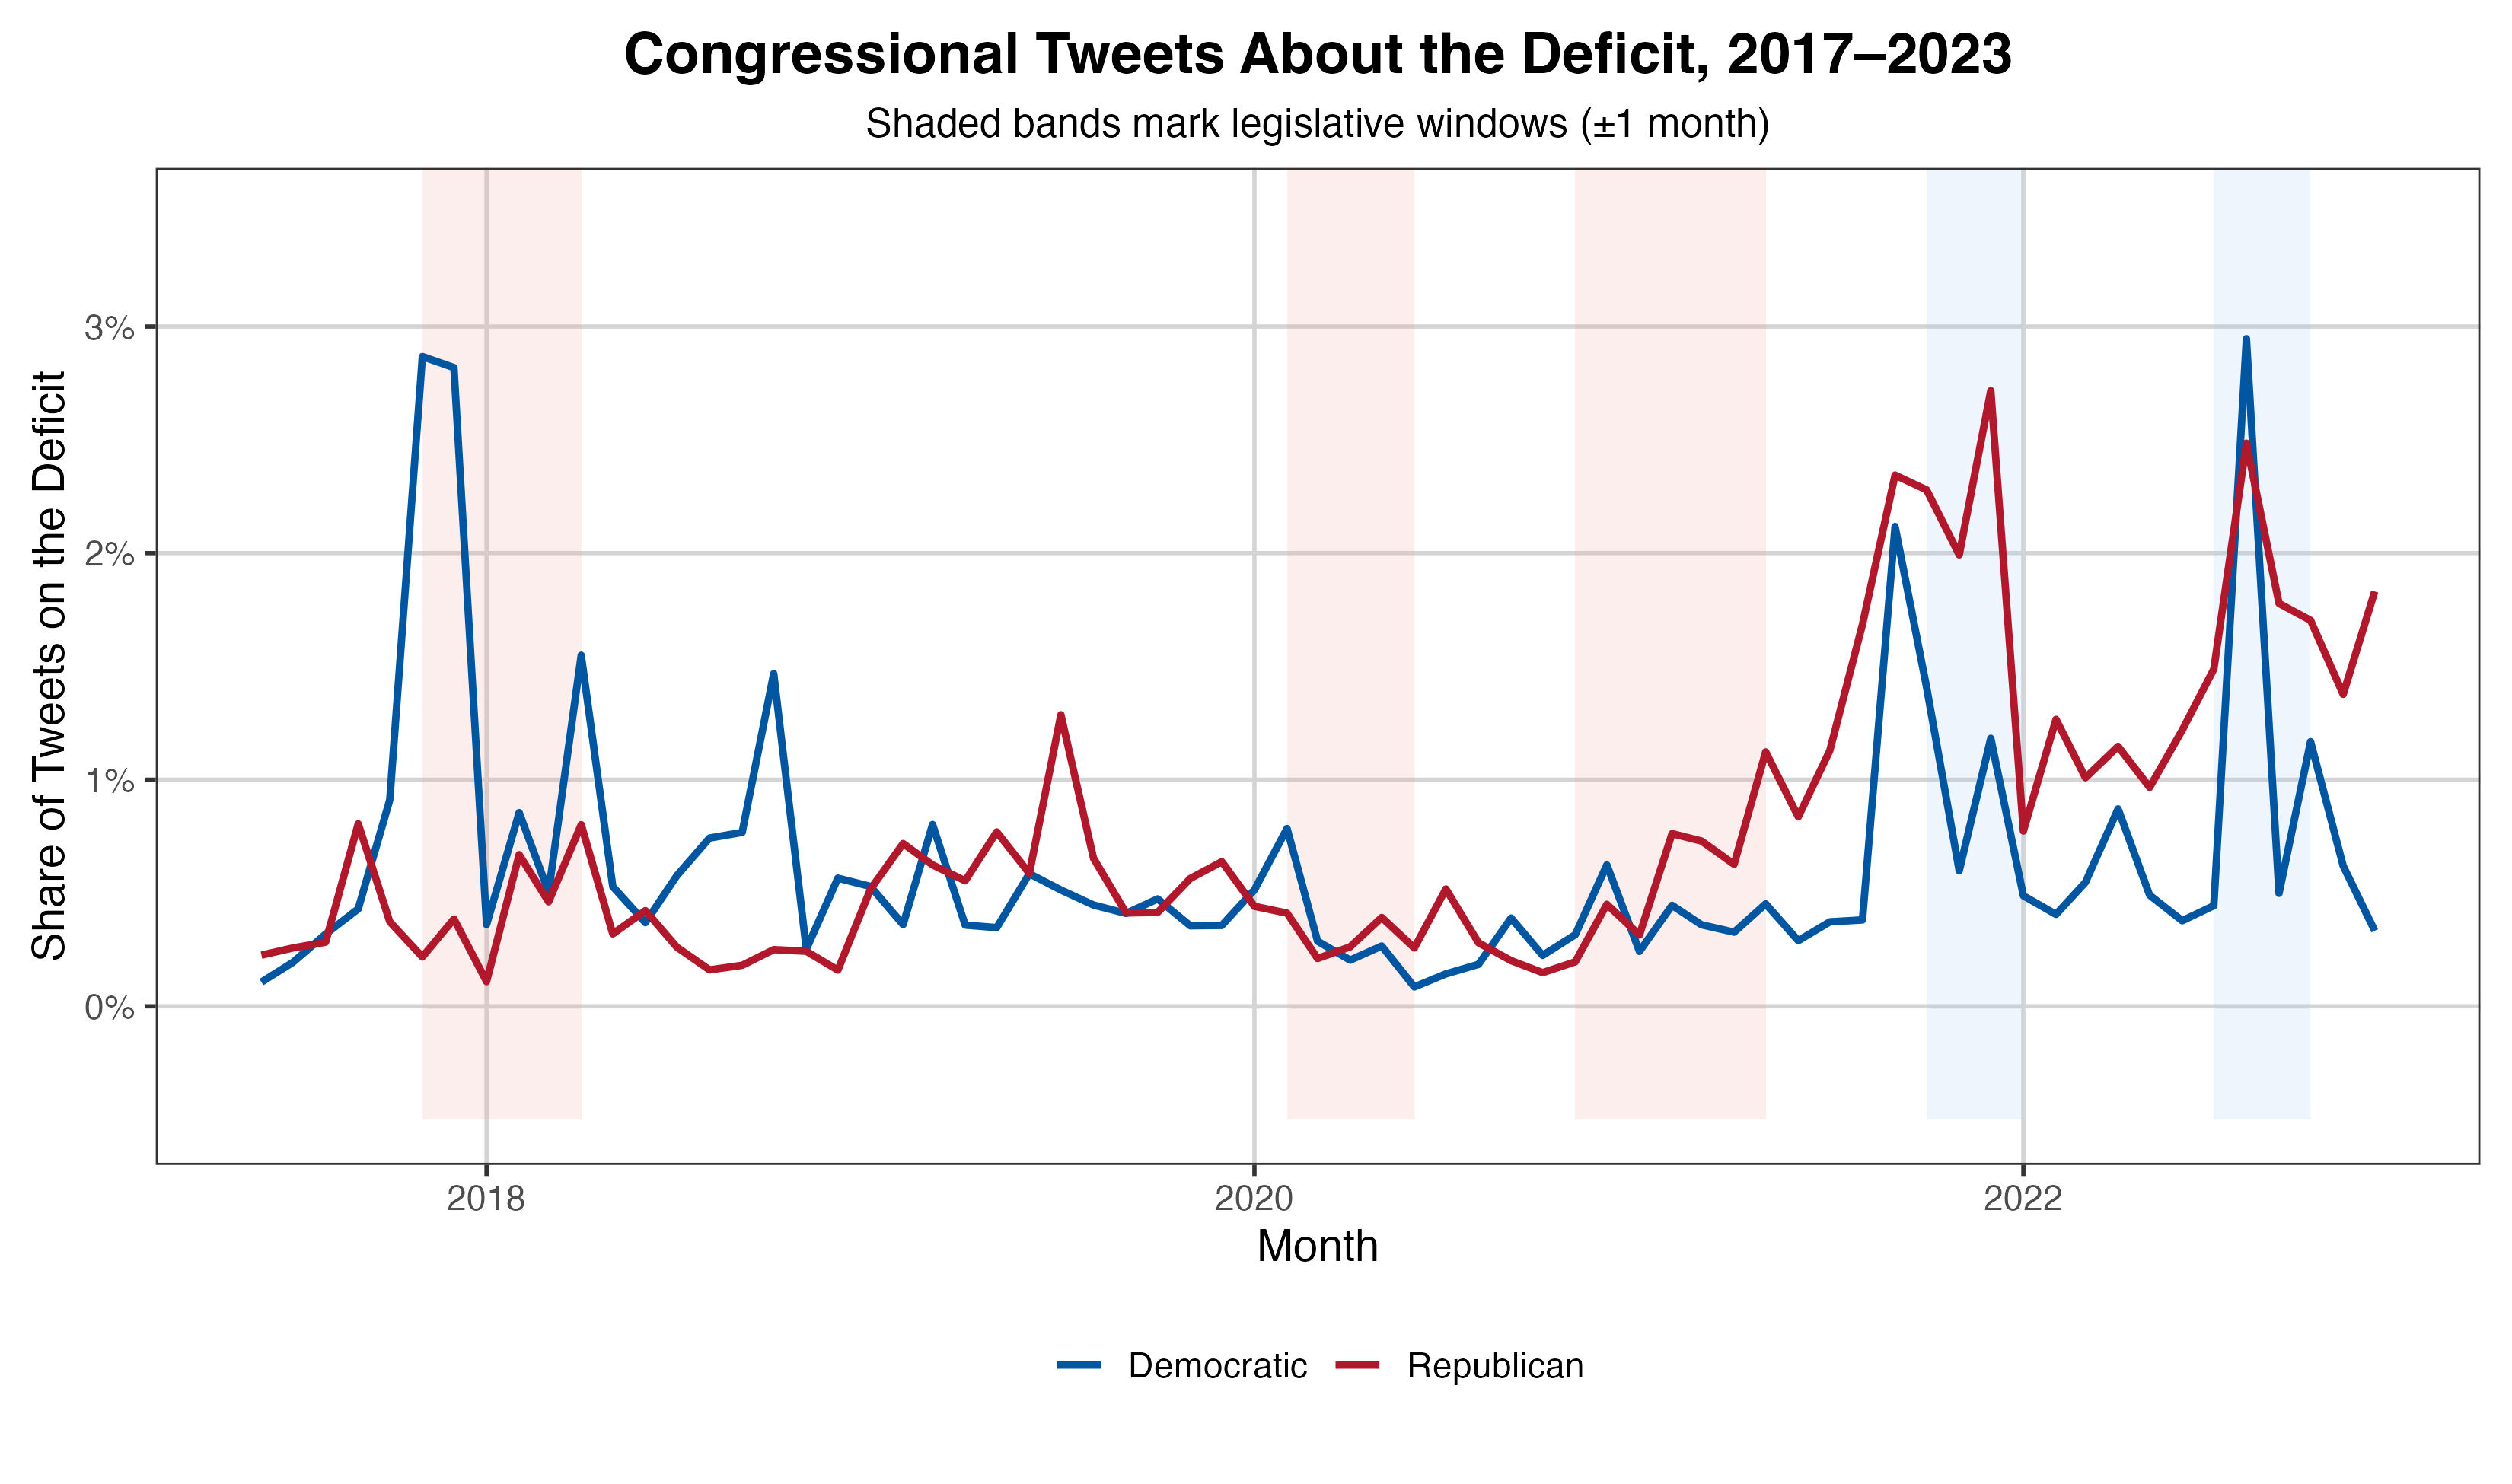
\includegraphics[width=0.85\textwidth,height=\textheight]{../figures/summary/deficit_tweet_share_with_legislation.png}

}

\caption{\label{fig-timeseries}Share of congressional tweets about the
deficit}

\end{figure}%

Figure~\ref{fig-timeseries} shows the monthly share of congressional
deficit tweets, by party, from June 2017 to January 2023. Consistent
with best practices in political science, this paper will represent the
Republican Party with red shading and the Democratic Party with blue.
Shaded areas indicate legislative periods -- defined as the month
before, during, and after the passage of a fiscally significant bill.
Legislative periods exclude small appropriations, procedural votes, and
commemorations.

The baseline deficit tweeting share for both parties is low, generally
staying under \textbf{1\%} averaged across members across the six years,
with notable accelerations occurring around legislative periods.
Democratic tweeting patterns remain relatively consistent across the six
years, with three notable peaks, all during legislative periods:
December 2017 (Tax Cuts and Jobs Act), October 2021 (Infrastructure
Investment and Jobs Act), and August 2022 (Inflation Reduction Act,
CHIPS \& Science Act). Republicans, however, demonstrate consistently
higher deficit tweeting rates as the minority party, as illustrated in
the peaks (2022, 2023) compared to relatively low rates from 2017-2021.

\section{Economic Indicators}\label{economic-indicators}

\begin{figure}

\centering{


\includegraphics[width=0.85\textwidth,height=\textheight]{../figures/economic_indicators/deficit_share_vs_inflation_smoothed.png}

}

\caption{\label{fig-deficit-vs-cpi}Deficit tweet share vs.~U.S. CPI
inflation.}

\end{figure}%

\FloatBarrier

Figure~\ref{fig-deficit-vs-cpi} plots deficit tweet share against US CPI
inflation (YOY) reveals a relatively strong positive relationship, as
indicated by its large r-value \textbf{(.78)}. There are a few plausible
explanations for this linear relationship. First, the elevated inflation
rates of 2022, peaking at \textbf{9.1\%} in June(40-year high), may have
increased elected officials concern about deficit spending. Public
discontent over higher prices may have also pressured representatives to
take a more hawkish approach on federal expenditures.

Another explanation could be that along with higher inflation, the
significant fiscal legislation being proposed in the summer of 2022 (eg,
IRA, CHIPS) may have drawn concerns from representatives prompting more
congressional tweets on the topic.

\section{Member-Level Patterns}\label{member-level-patterns}

\begin{figure}[H]

\centering{

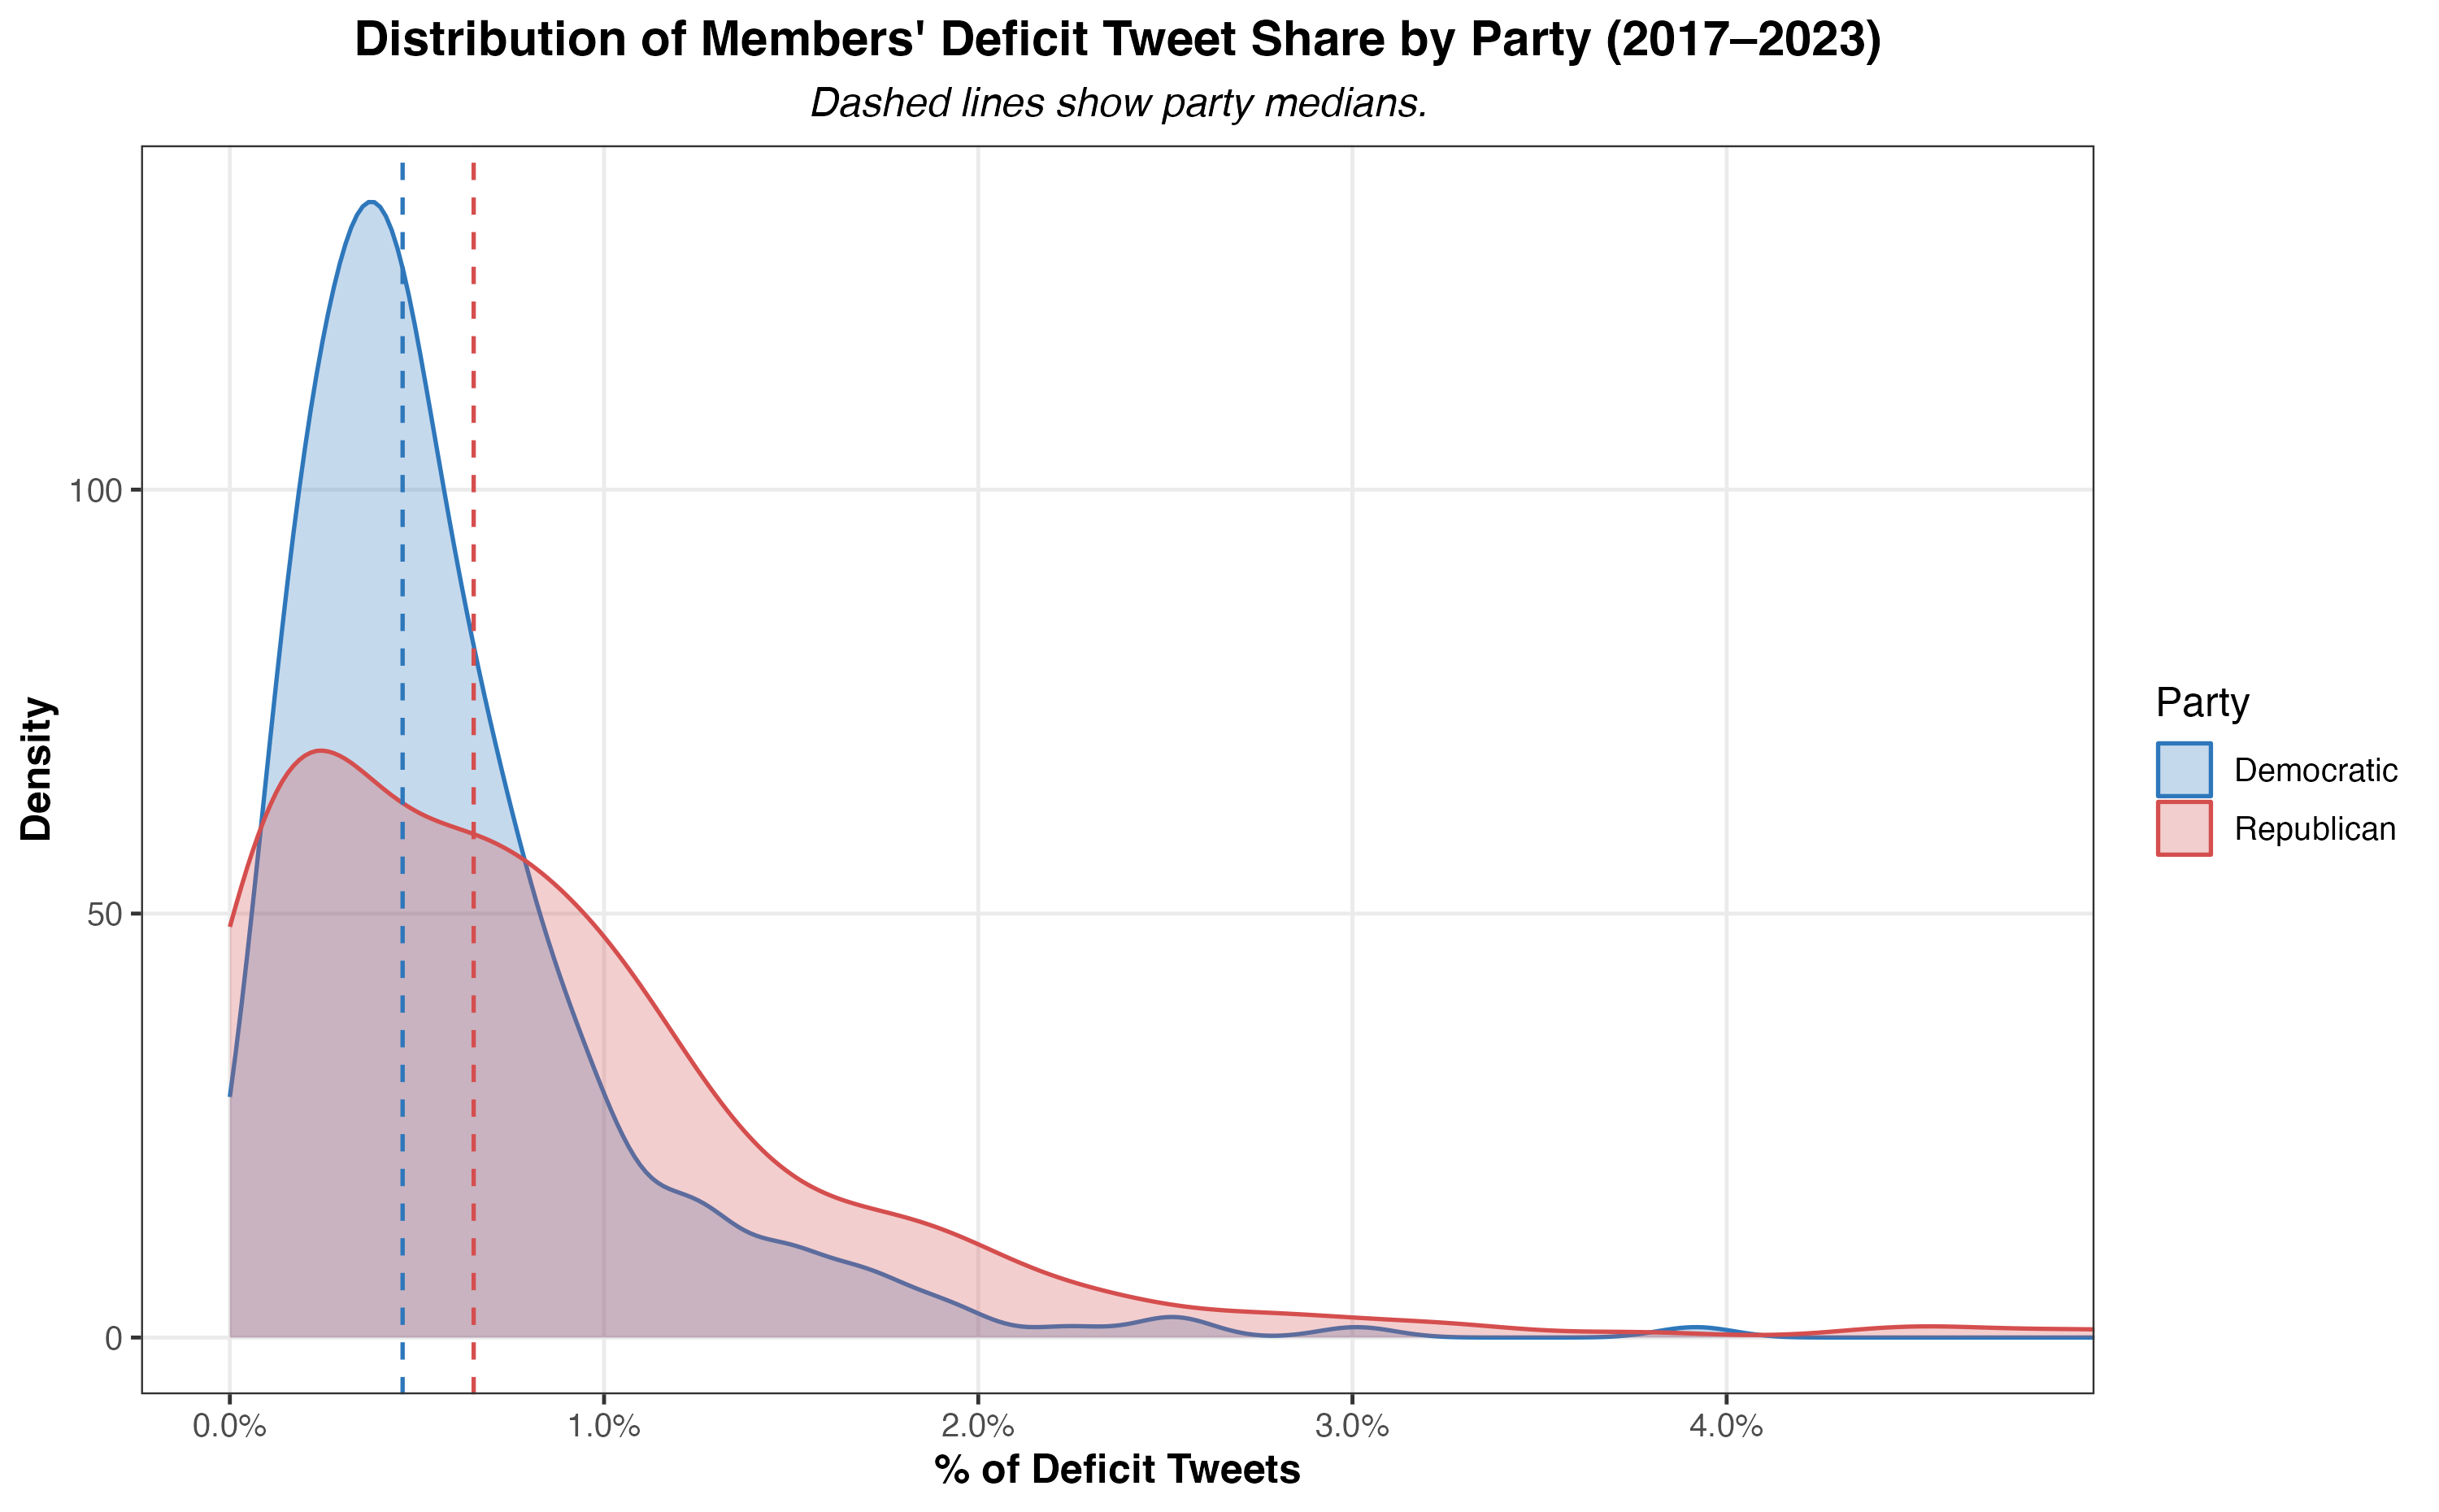
\includegraphics[width=0.75\textwidth,height=\textheight]{../figures/individuals/density_pct_deficit_by_party_overall.png}

}

\caption{\label{fig-member-share-by-party}Share of deficit tweets by
party (member-level distribution).}

\end{figure}%

\FloatBarrier

Figure~\ref{fig-member-share-by-party} presents member-level
distributions of deficit tweeting, calculated as the share of each
member's tweets that mention the deficit over the entire period. As
illustrated by the dashed lines (party medians), Republicans tweet about
the deficit more frequently than Democrats, with average shares of
\textbf{0.81\%} and \textbf{0.62\%}, respectively.

Democrats display a relatively compact distribution, with most
representatives falling below \textbf{0.7\%}, indicating less
inter-party variation in deficit tweeting. Republicans, however, show
far greater variability within their party. The GOP's right tail
distribution illustrates that, compared to their Democratic colleagues,
a far greater proportion of of members tweet about the deficit at much
higher rates, with outliers reaching \textbf{4--8\%}.

\begin{figure}

\centering{

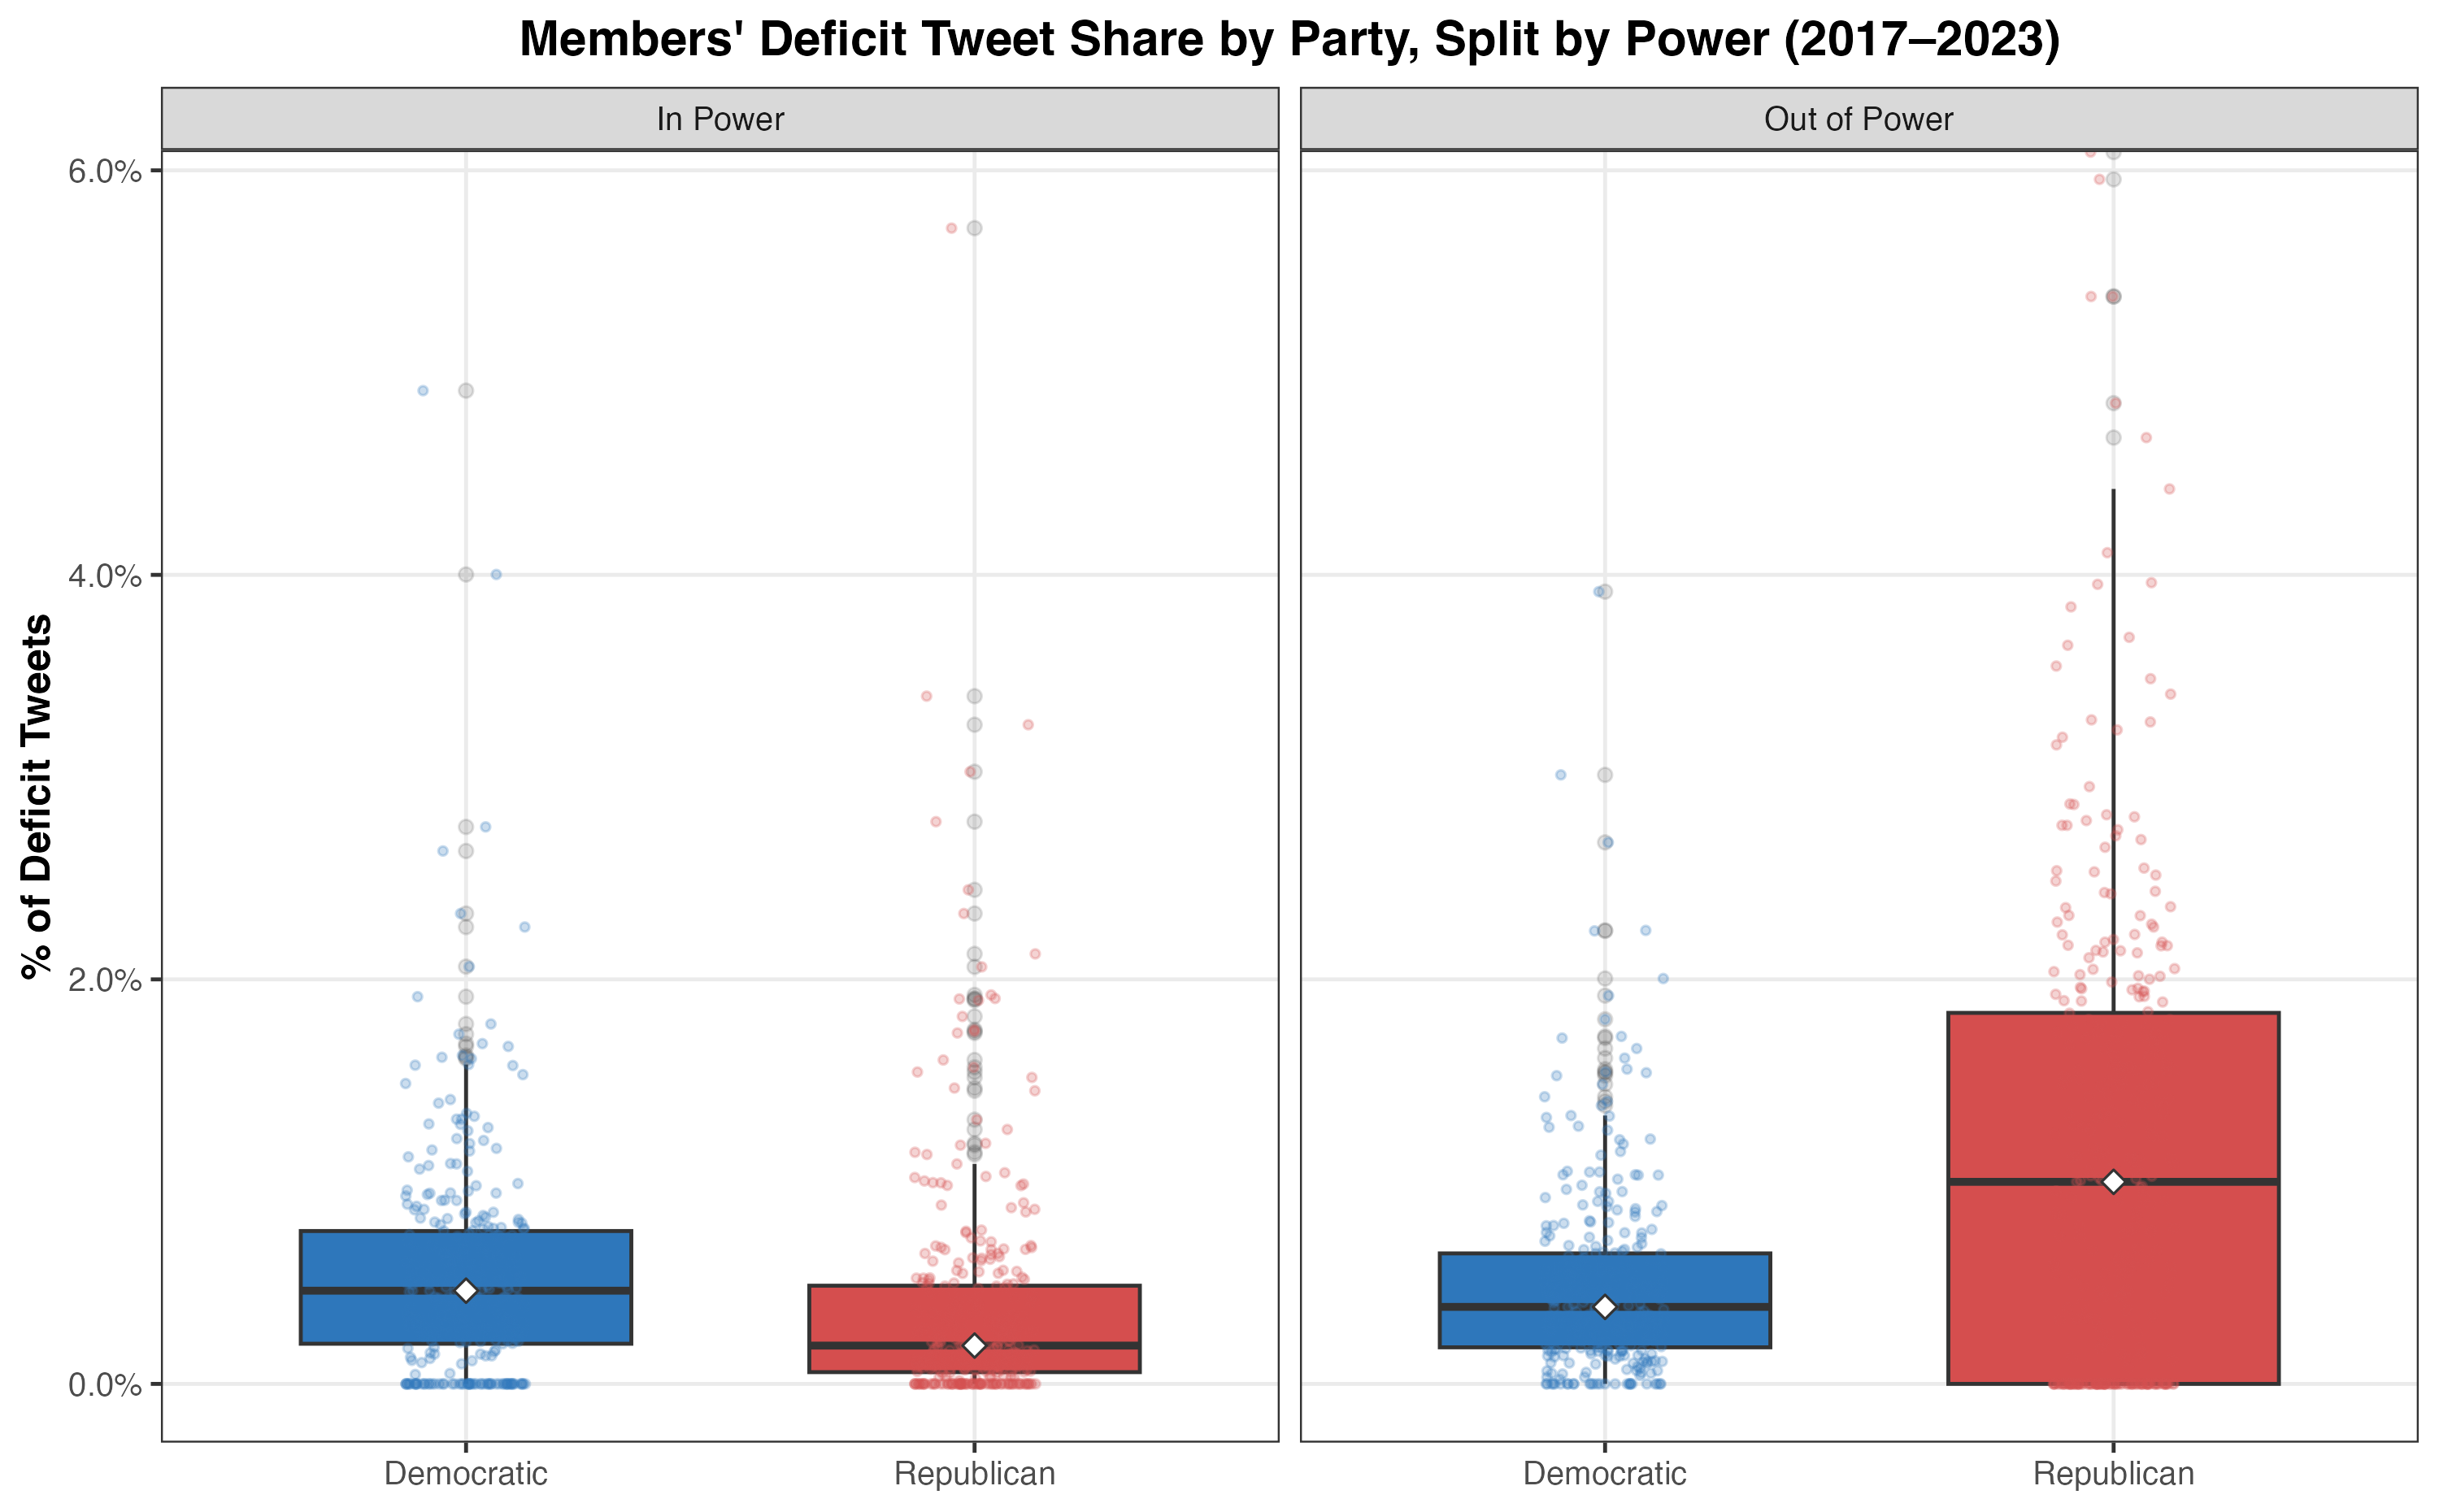
\includegraphics[width=0.85\textwidth,height=\textheight]{../figures/individuals/box_party_split_by_power.png}

}

\caption{\label{fig-power-boxplot}Distribution of deficit tweets by
power (boxplot).}

\end{figure}%

\FloatBarrier

Figure~\ref{fig-power-boxplot} breaks down these distributions further
by institutional power status (majority vs.~minority). The left and
right panels juxtapose the distribution when a member's party controls
the presidency (in-power) versus when it does not (out-of-power). For
instance, Democrats would be considered in-power from January 2021 to
January 2023 under President Joe Biden, while Republicans would be
out-of-power during this same period.

Figure~\ref{fig-power-boxplot} shows a clear asymmetry in GOP tweeting
patterns between these periods. When moving between power contexts, the
GOP median tweet share increases five-fold \textbf{0.2\% to 1.0\%} and
the inter-quartile range from \textbf{0.6\%} to \textbf{1.8\%}. In other
words, Republicans were far more likely to tweet about the deficit under
President Biden than under President Trump. This stark distributional
contrast illustrates a synchronized and cohesive shift in messaging
among Republicans: emphasize the deficit more in periods of political
weakness. Democrats, by contrast, remain relatively stable across
contexts and actually demonstrate a modest increase in spread and
averages when in power. \FloatBarrier

\begin{figure}

\centering{

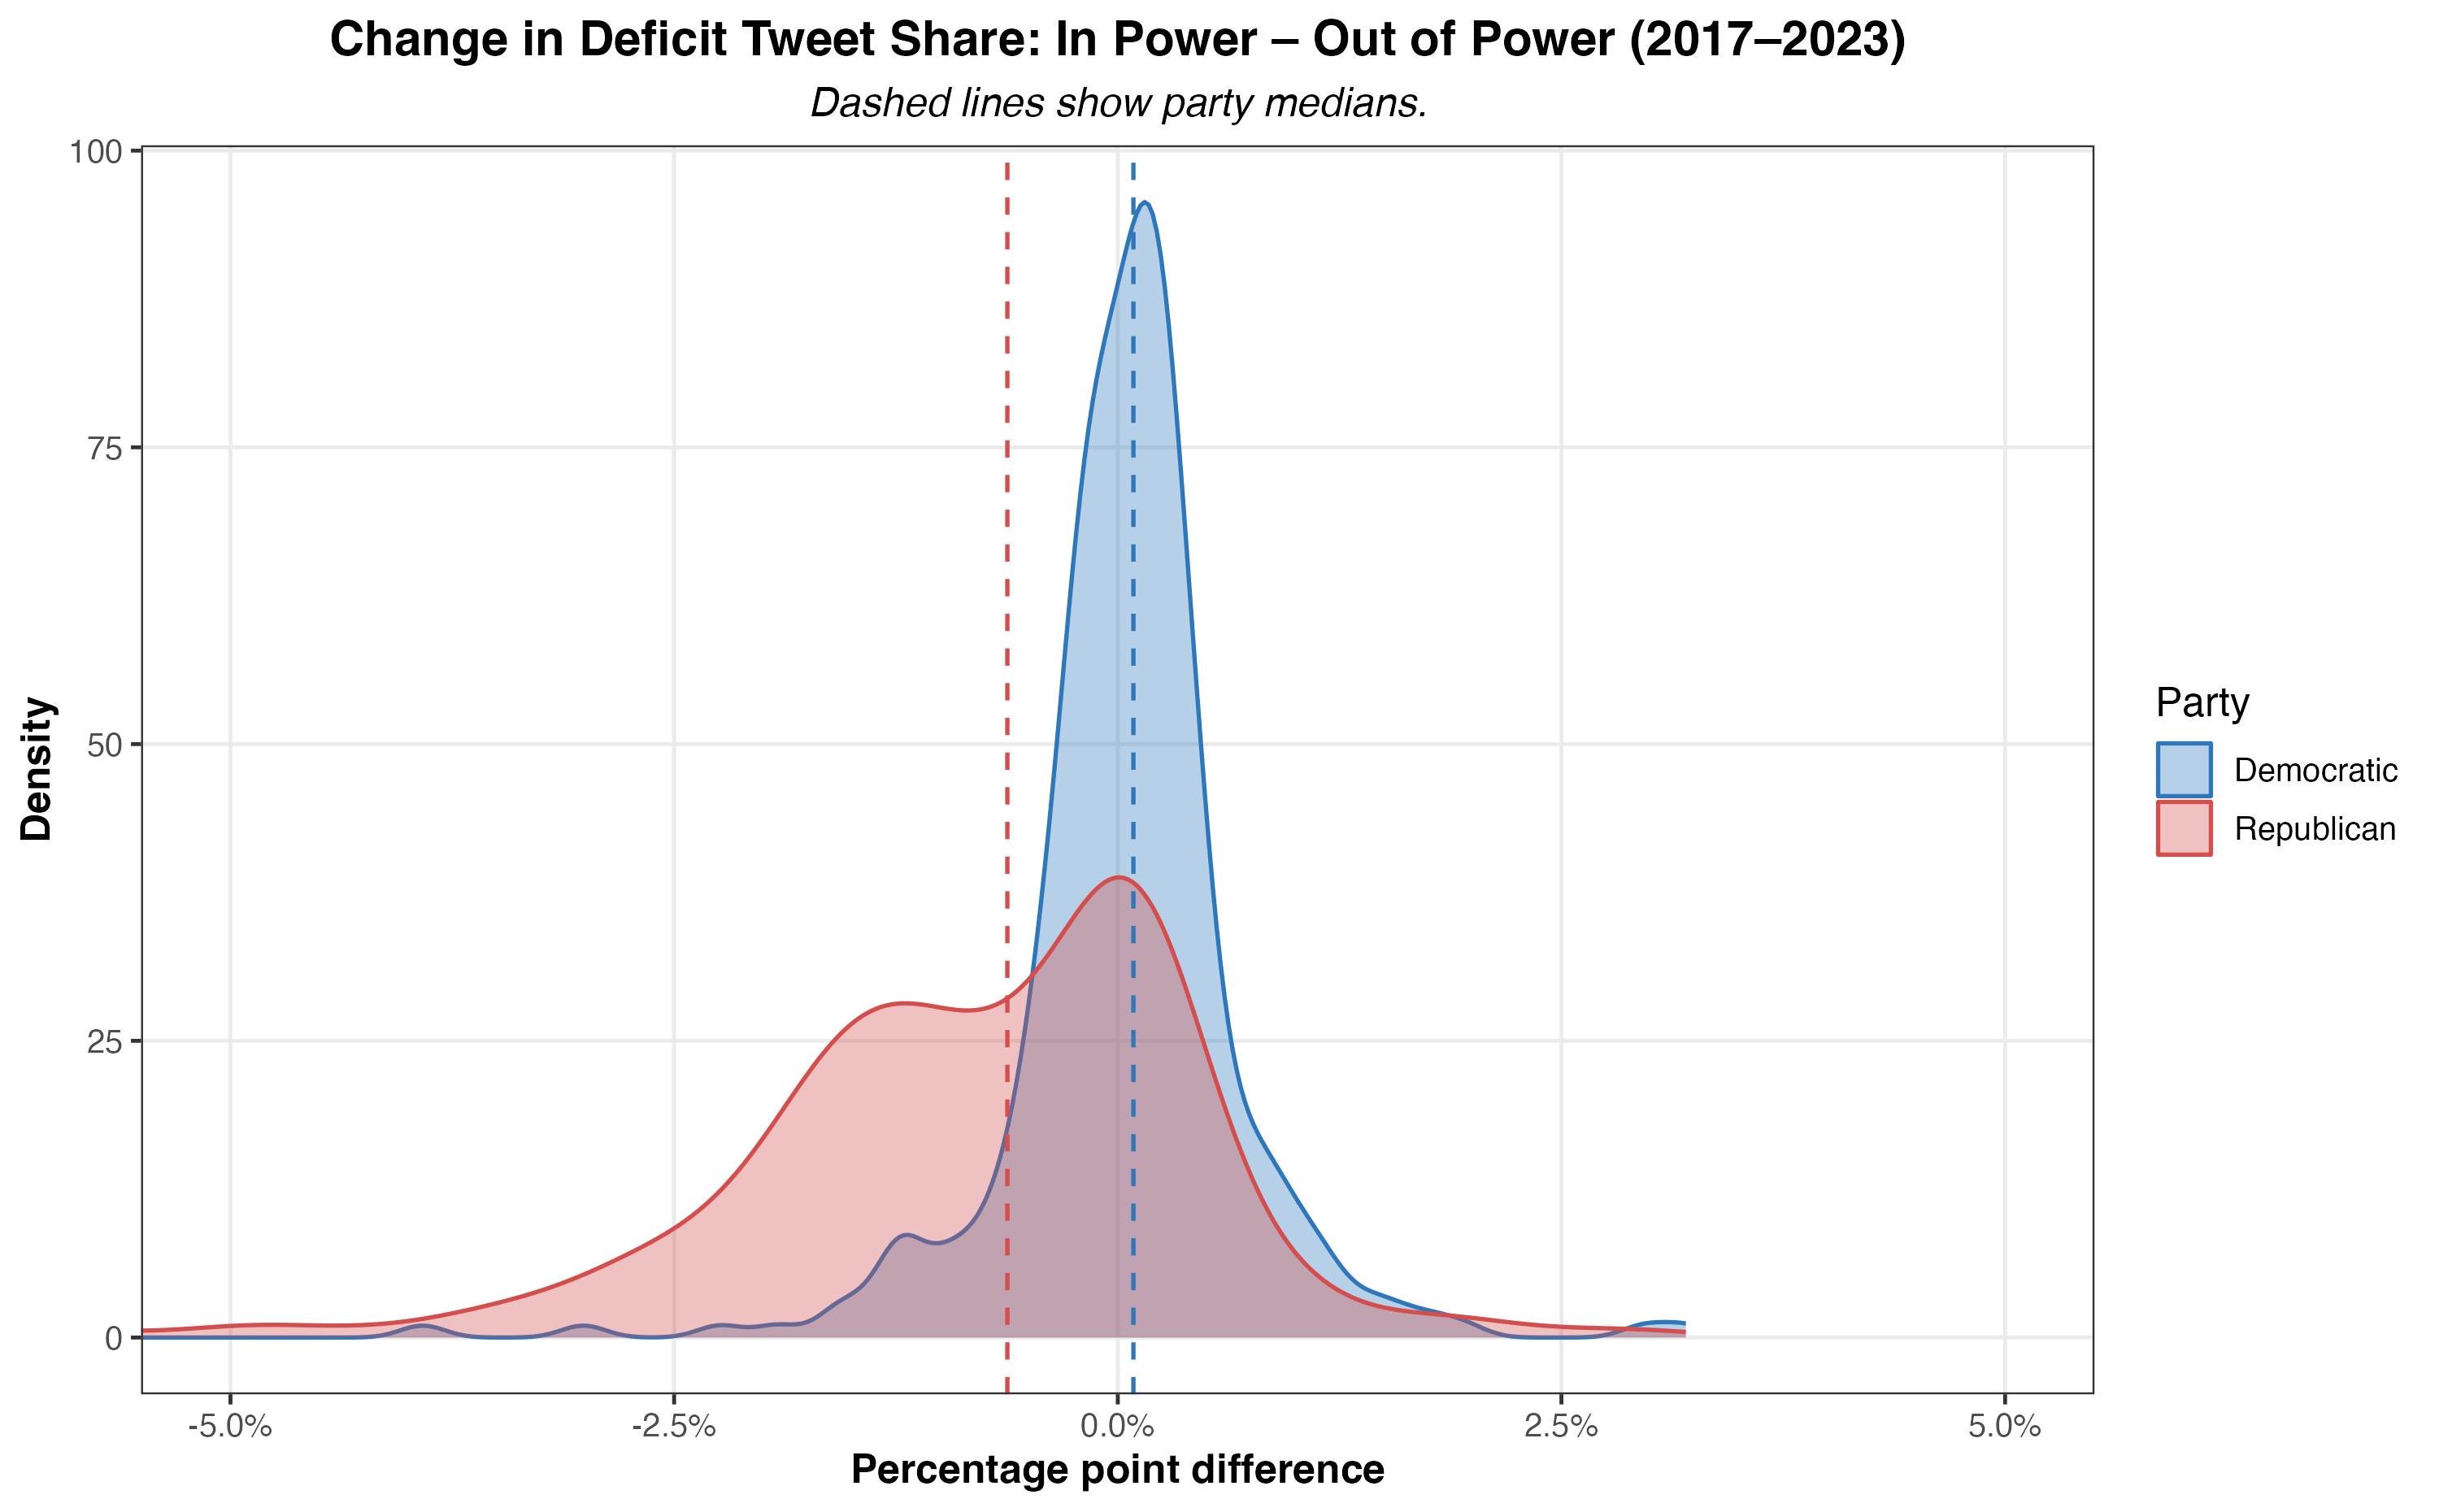
\includegraphics[width=0.85\textwidth,height=\textheight]{../figures/individuals/density_in_minus_out_overlay.png}

}

\caption{\label{fig-inout-shifts}In--out shifts in deficit tweeting
(histogram).}

\end{figure}%

\FloatBarrier

Figure~\ref{fig-inout-shifts} visualizes these shifts more directly by
plotting the distribution of changes in deficit tweeting when moving
from in-power to out-of-power contexts. The x-axis represents the
difference in deficit tweet share between these two periods for each
member (in minus out). Positive values indicate that a member tweeted
more about the deficit when in power, while negative values indicate
higher tweeting rates when out of power. The GOP's comprehensive party
shift, highlighted is evident, with the bulk of their parties
distribution skewed negatively.

Taken together, Figure~\ref{fig-power-boxplot} and
Figure~\ref{fig-inout-shifts} suggest that Republicans are far more
sensitive to power status when deciding how frequently to tweet about
the deficit, while Democrats maintain a more consistent messaging
strategy regardless of institutional control. These results illustrate a
broader point about the coordination of modern political communication
strategies on Twitter. The pronounced and systematic increase in
Republican deficit tweeting supports the notion of uniform, top-down
messaging within parties.

\section{Leadership Analysis}\label{leadership-analysis}

\begin{figure}[H]

\centering{


\includegraphics[width=0.75\textwidth,height=\textheight]{../figures/leadership/leader_deficit_tweets.png}

}

\caption{\label{fig-leadership}Deficit tweeting by congressional leaders
(House and Senate; majority vs.~minority roles).}

\end{figure}%

\FloatBarrier

Figure~\ref{fig-leadership} summarizes deficit tweeting among House and
Senate leaders in both majority and minority roles. Tweeting patterns
vary by party and institutional position, with the sharpest contrasts
appearing in the Senate. Senator Chuck Schumer tweeted about deficits
far more often as Majority Leader \textbf{4.0\%} than as Minority Leader
\textbf{1.0\%}, while Senator Mitch McConnell showed the reverse,
posting more in the minority \textbf{1.9\%} than the majority
\textbf{0.05\%}. Notably, in contrast to Senate counterpart, Speaker
Nancy Pelosi displayed higher rates in the minority \textbf{1.1\%} than
as Speaker \textbf{0.5\%}. Representative McCarthy's abnormally small
number of registered tweets (762), suggest a potential issue in
reconciling changes in his twitter handle. Considering congressional
leaders often maintain multiple twitter accounts, with new handles
introduced and changed depending on their relative power status
(majority, minority, rank-and-file), some of Representative McCarthy's
twitter accounts may have not been picked up by the data.

Representative Paul Ryan - a self-proclaimed ``deficit hawk'' and
speaker of the House from 2017-2019 - is an central political figure in
discourse surrounding the national deficit. Speaker Ryan, whose deficit
tweet share is just \textbf{0.17\%}, has been long criticized for his
messaging around the national debt - which often conflict with his
historical voting patterns towards fiscally significant bills.

A 2018 Politico op-ed \emph{Paul Ryan's Legacy of Red Ink} writes ``Ryan
loves to \emph{talk} about reducing the national debt, but what he loves
to \emph{do} is reduce taxes, which increases the national debt''. My
research highlights an important nuance to this point. While Speaker
Ryan may emphasize the deficit in out-of-power contexts, he does not
tweet about the deficit in periods of legislative control. Ryan's
deficit aprehesnsions may be due to his legislative agenda during this
period, passing the Tax Cuts and Jobs Act (2017), which, by CBO
estimates, will balloon the national debt by \$1.5 Trillion over the
following decade. Further analysis of Speaker Ryan's tweeting habits,
especially in instances of minority power, would help clarify his
communication patterns, and the degree to which he uses the federal
deficit as a tool for partisan ends. Nonetheless, this research confirms
an important point about the messaging strategy of a key American
legislator: Paul Ryan, a self-identified ``fiscal conservative'', rarely
mentioned the deficit when holding complete legislative control from
2017 to 2019.

Aside from highlighting rhetoric patterns in key legislators,
@fig-leadership also underscores a broader point about communication
uniformity among party leaders and rank-and-file represenatives.
Previous research establishes the growing polarization in congressional
ideology and party-line voting over recent decades (CQ Roll Call 2024).
My research provides insight into the specific polarities of a single
rhetorical subject - the federal deficit.

For Democrats, the divergent tweeting patterns of Speaker Pelosi and
Senator Schumer suggest a compartively weaker inter-party alignment in
messaging. These patterns are consistent with the broader Democratic
caucus, which show no discernible difference in deficit tweeting between
power contexts (as shown in Figure~\ref{fig-power-boxplot} and
Figure~\ref{fig-inout-shifts}).

The GOP, however, presents a more uniform party dynamic. Senator
McConnell's significant increase in deficit tweeting in out of power
contexts mirrors the broader Republican trend illustrated in
Figure~\ref{fig-inout-shifts}. The two messaging strategies employed by
party leaders reflect a broader division in party dynamics between
Democrats and the GOP. Democratic leaders' deficit messaging is not tied
to or correlated with their power status within the party. Republicans,
by contrast, demonstrate higher levels of systematic and uniform shifts
in messaging between power contexts.

\FloatBarrier

\section{Legislative Context}\label{legislative-context}

\begin{figure}[H]

\centering{


\includegraphics[width=0.75\textwidth,height=\textheight]{../results/tweetlevel_deficit_share_by_party.png}

}

\caption{\label{fig--deficit-share-by-party}Deficit share within
legislative windows, by party.}

\end{figure}%

\FloatBarrier

Legislative periods -- defined by one month before and after bill
passage -- raise the conditional rate modestly to \textbf{(0.9\%).}
Industrial policy bills -- the Inflation Reduction Act (IRA) and CHIPS
Act, passed under President Biden -- generated the highest levels of
deficit tweeting \textbf{(1.6\%)} among passed legislation. The Tax Cuts
and Jobs Act (2017), passed under President Trump, had a deficit tweet
share of \textbf{(1.2\%)} -- higher than baseline, but lower than the
IRA/CHIPS.~

@fig--deficit-share-by-party decomposes these differences by party. At
baseline, Republicans tweet about the deficit more often
\textbf{(0.8\%)} than Democrats \textbf{(0.6\%)} -- a gap that persists
across most legislative windows. During the IRA and CHIPS periods,
Republicans' tweets accelerated, with deficit mentions at nearly
\textbf{(2.0\%)}, compared to \textbf{(1.3\%)} among Democrats. However,
the TCJA -- a partisan GOP tax cut-- is a noticeable and stark
exception. During these three months, the Democrats' deficit share
spikes to \textbf{(2.0\%)}, while the Republicans' share falls to just
\textbf{(0.2\%)}, reflecting a partisan realignment around a highly
divisive bill. In contrast, during the COVID relief period in 2020 -- a
non-partisan voting context -- both parties converged at very low levels
\textbf{(0.3--0.4\%)}.

\FloatBarrier

\section{Regression Visualization}\label{regression-visualization}

The following regression models offer a structured approach to examining
how institutional, fiscal, and partisan contexts affect the likelihood
of congressional deficit tweeting.

Since the specifications rely heavily on interaction terms, it is useful
to provide a framework for their interpretation first. The coefficients
are expressed as odds ratios: values above one indicate that Republicans
are more likely to tweet about deficits relative to Democrats. In
contrast, values below one indicate a narrowing of the GOP-Dem gap. Each
model includes majority interaction coefficients of the general form GOP
× Conditioning Variable. These coefficients indicate whether the
baseline Republican--Democratic difference changes under specific
conditions (legislative windows, presidential control, chamber control,
or trifectas).

\begin{figure}[H]

\centering{


\includegraphics[width=0.75\textwidth,height=\textheight]{../results/good_tables/r3_legislative_windows_main.png}

}

\caption{\label{fig-r1-legislative-windows}Regression 1: Legislative
windows.}

\end{figure}%

\FloatBarrier

The baseline model, Figure~\ref{fig-r1-legislative-windows}, examines
partisan differences in legislative periods without conditioning on
institutional control. The non-significant results suggest that, when
averaged across both Democratic and Republican presidencies, legislative
windows themselves do not systematically impact the partisan gap in
deficit tweeting.

\FloatBarrier

\begin{figure}[H]

\centering{


\includegraphics[width=0.75\textwidth,height=\textheight]{../results/good_tables/r5_majority_context_main.png}

}

\caption{\label{fig-r2-presidency}Regression 2: Majority context
(presidency).}

\end{figure}%

\FloatBarrier

Figure~\ref{fig-r2-presidency}, which controls for presidential party,
substantially changes the results from the preceding specification.

Republicans' odds of tweeting about deficits are nearly double
\textbf{(OR = 1.87)} when not holding the presidency compared to
Democrats under the same condition. In contrast, \textbf{GOP ×
Legislative window (OR = 0.38)} highlights that under a Republican
presidency, the partisan gap narrows during legislative months; the odds
of the GOP tweeting are \textbf{62\%} lower than those of Democrats.
This pattern aligns with Figure~\ref{fig-timeseries}, which shows that
Republican tweeting contracts while Democratic tweeting spikes as
Congress passes the Tax Cuts and Jobs Act in late 2017. However, the
three-way interaction coefficient \textbf{GOP × Legislative window ×
Minority presidency} reveals a reversal of this trend \textbf{(OR =
4.24)}. Under a Democratic presidency, Republicans' odds of tweeting are
more than four times higher than those of Democrats in the same
condition.

\FloatBarrier

\begin{figure}[H]

\centering{


\includegraphics[width=0.75\textwidth,height=\textheight]{../results/good_tables/r6_majority_context_combos.png}

}

\caption{\label{fig-r3-chamber-presidency}Regression 3: Majority context
--- chamber and presidency combinations.}

\end{figure}%

\FloatBarrier

The third model further examines the role of institutional power by
including combinations of chamber control. The regression baseline is
Democrats, outside legislative windows, when their party controls
nothing (i.e., a minority in the House and Senate; does not hold the
Presidency).

\textbf{GOP x Legislative window (OR = 0.31)} indicates that during
legislative months, when holding a trifecta, Republicans' odds of
tweeting are \textbf{69\%} lower than Democrats. The Tax Cuts and Jobs
Act (2017) -- a legislative window under a GOP trifecta -- is an
illustration of this circumstance. Once again, once we condition on a
Democratic trifecta, this effect reverses. Relative to the baseline
condition (a GOP trifecta), Republicans' odds of deficit tweeting are
seven times higher than those of Democrats in the same context. The
juxtaposition of these two coefficients \textbf{(OR = 0.31)} versus
\textbf{(OR = 7.00)} illustrates that legislative timing by itself isn't
determinative of tweeting gaps -- but who governs is. Under Democratic
control (i.e., 2021-2023), Republicans accelerate deficit rhetoric
during legislative months, while under the GOP trifecta (i.e.,
2017-2019), they significantly reduce deficit tweeting frequencies.

\subsection{\texorpdfstring{\textbf{Bill Partisanship and Fiscal
Magnitude}}{Bill Partisanship and Fiscal Magnitude}}\label{bill-partisanship-and-fiscal-magnitude}

Across all three specifications, the coefficients for Fiscal magnitude
(z) remain consistently insignificant (\textasciitilde1.0).~ These
coefficients, based on a normalized measure of a given bill's 10-year
CBO estimate, suggest that the fiscal consequences of policy do not
systematically impact partisan tweeting gaps.

Bill partisanship (z), however, shows significant contractions in the
GOP-Dem tweeting gap once institutional control is included \textbf{(OR
\textasciitilde{} 0.50)}. In other words, for each one-SD increase in a
bill's partisanship score, the GOP-Dem gap contracts by roughly half.
Notably, because these variables are continuous (ie, z-scores), the
coefficients represent slopes rather than a baseline-specific effect.
For example, in the context of bill partisanship, if Republicans are
twice as likely as Democrats to tweet at \textbf{z = 0 (OR = 2.0)}, that
gap narrows to parity at \textbf{z = 1 (OR = 1.0).}

\FloatBarrier




\end{document}
